\documentclass[aspectratio=169, table]{beamer}

\usepackage[utf8]{inputenc}
\usepackage{listings} 

\usetheme{Pradita}

\subtitle{MTI104 - IT Services}

\title{Session-01:\\\LARGE{Practices to Manage Releases\\}}
\date[Serial]{\scriptsize {PRU/SPMI/FR-BM-18/0222}}
\author[Pradita]{\small{\textbf{Alfa Yohannis}}}

\begin{document}

\frame{\titlepage}

\begin{frame}
	\frametitle{Introduction to the Cycle}
	\begin{itemize}
		\item Cycle starts with design, followed by build, test, and transition.
		\item Transition involves moving a built object into production.
		\item Streamlined process needed for moving packages to higher environments.
		\item Policies, principles, and processes guide releases.
		\item Technical aspect of moving packages to minimize risks.
		\item Releases in the waterfall world happened infrequently.
		\item Process of development and testing was the focus.
	\end{itemize}
\end{frame}

\begin{frame}
	\frametitle{Changes in DevOps Industry}
	\begin{itemize}
		\item In DevOps, releases and deployments happen frequently.
		\item Automation is key to seamless activities.
		\item Speed is crucial; blockers are to be eliminated.
		\item Release management and deployment management are critical practices.
		\item ITIL 4 emphasizes separate practices for release and deployment.
		\item Depth of knowledge is essential despite examination requirements.
		\item Exam tip: Expect questions on release and deployment practices.
	\end{itemize}
\end{frame}

\begin{frame}
	\frametitle{Release Management Overview}
	\begin{itemize}
		\item Release management spans development and operations.
		\item ITIL defines a release as a version of a service or configuration item.
		\item Developed in lower environments and tested in higher environments.
		\item Testing can be manual or automated.
		\item Software moved to production as a release.
		\item Releases may include software, break-fixes, and hardware changes.
		\item Releases are often packaged to minimize production disruptions.
	\end{itemize}
\end{frame}

\begin{frame}
	\frametitle{Change Control vs. Release Management}
	\begin{itemize}
		\item Change control: obtaining approvals and controlling changes.
		\item Release management: managing technical aspects of changes.
		\item Release management includes requirement gathering, coding, testing, deployment.
		\item Change control ensures development efforts aren't wasted.
		\item Change control also modifies solutions if needed.
		\item Release management handles overall planning and execution.
		\item Change control provides oversight before production changes.
	\end{itemize}
\end{frame}

\begin{frame}{Change control vs. release management}
	 \frametitle{Change control vs. release management}
\begin{center}
	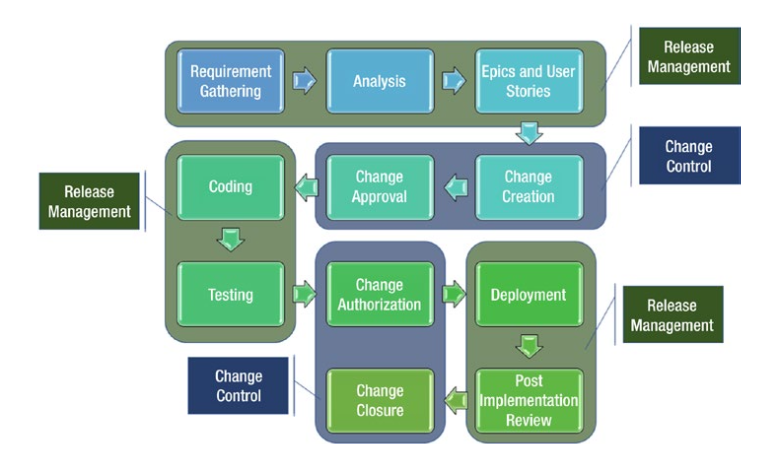
\includegraphics[width=0.8\linewidth]{images/image-01.png}
\end{center}
\end{frame}

\begin{frame}
	\frametitle{Release Fundamentals}
	\begin{itemize}
		\item Releases include hardware and software components.
		\item Training and documentation updates are part of the release.
		\item Third-party components may be included in releases.
		\item Release scope is broad, covering all service components.
		\item Major releases involve significant business impact.
		\item Minor releases are frequent and less risky.
		\item Emergency releases are used to fix critical incidents.
	\end{itemize}
\end{frame}

\begin{frame}
	\frametitle{Release Scheduling and Reviews}
	\begin{itemize}
		\item Releases can be scheduled or ad hoc.
		\item Emergency releases address critical issues.
		\item Periodic releases provide predictability for businesses.
		\item DevOps promotes modular, frequent releases.
		\item Release schedule aligns with change schedule.
		\item Release reviews identify lessons learned and improve future releases.
		\item Waterfall vs. Agile/DevOps approaches differ in release management.
	\end{itemize}
\end{frame}

\begin{frame}{Waterfall vs. Agile/DevOps releases}
	 \frametitle{Waterfall vs. Agile/DevOps releases}
\begin{center}
	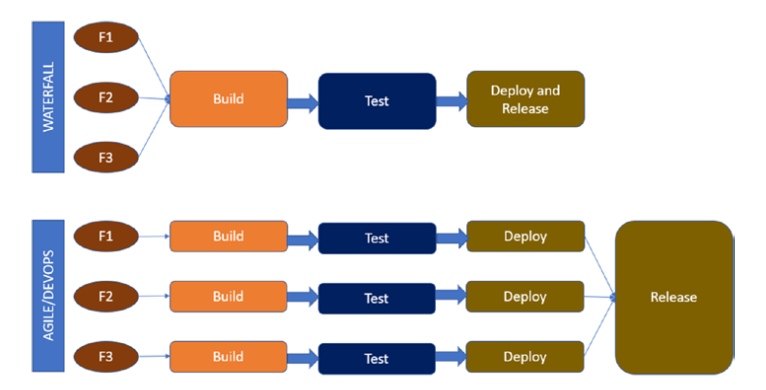
\includegraphics[width=0.8\linewidth]{images/image-02.png}
\end{center}
\end{frame}

\begin{frame}
	\frametitle{Release Management in Agile/DevOps}
	\begin{itemize}
		\item Agile/DevOps: release management becomes iterative.
		\item Release planning aligns with Agile Release Trains (ARTs).
		\item Continuous deployment adapts release management to frequent deployments.
		\item Continuous delivery combines iteration with traditional deployment.
		\item Release management ensures stable paths to production.
		\item Release management in continuous delivery provides control.
		\item Maturity leads to a preference for continuous deployment.
	\end{itemize}
\end{frame}

\begin{frame}
	\frametitle{Release Management Techniques}
	\begin{itemize}
		\item Techniques mitigate risks in stable environments.
		\item Proof of Concept (POC) tests the feasibility of major changes.
		\item POC ensures development and testing paths are viable.
		\item Pilot phase follows POC, testing functionality with real data.
		\item Pilot releases involve limited, controlled testing.
		\item Successful pilot further validates the chosen path.
	\end{itemize}
\end{frame}

\begin{frame}
	\frametitle{Blue–Green Release Overview}
	\begin{itemize}
		\item DevOps projects deploy without downtime
		\item Blue-green deployment runs two environments in parallel
		\item Environments designated as blue or green
		\item One environment is active, the other passive
		\item Active environment handles all user requests
		\item Passive environment deployed first
		\item Load balancer switches user requests to the updated environment
	\end{itemize}
\end{frame}

\begin{frame}{Blue-green release approach}
	 \frametitle{Blue-green release approach}
\begin{center}
	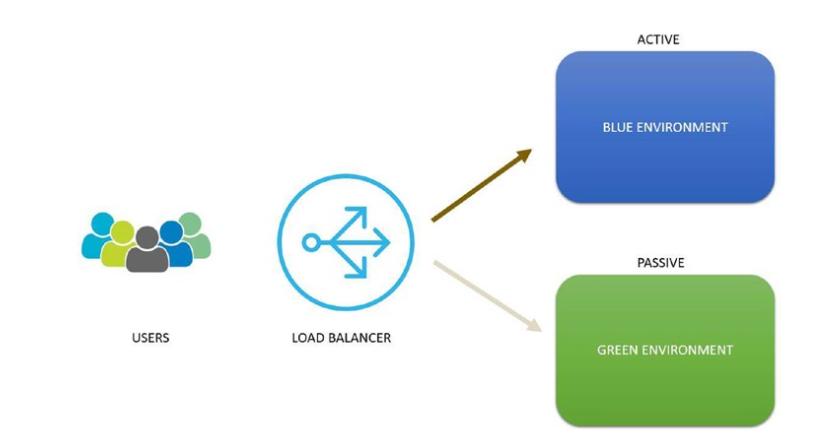
\includegraphics[width=0.8\linewidth]{images/image-03.png}
\end{center}
\end{frame}

% Slide 2: Blue–Green Release Example
\begin{frame}
	\frametitle{Blue–Green Release Example}
	\begin{itemize}
		\item Example: Blue is active, green is passive
		\item Green environment deployed without affecting users
		\item Once green is ready, switch user requests from blue to green
		\item Blue environment is updated next
		\item Both environments receive updates requiring downtime
		\item Users experience no downtime
		\item Load balancer manages user requests between environments
	\end{itemize}
\end{frame}

% Slide 3: Feature Toggles Overview
\begin{frame}
	\frametitle{Feature Toggles Overview}
	\begin{itemize}
		\item Software development technique to change features
		\item No code changes needed
		\item Branching technique used for feature development
		\item Features toggled on/off based on criteria
		\item Example: Features F1, F2, and F3 in a shopping portal
		\item Only F2 and F3 are live, F1 is toggled off
	\end{itemize}
\end{frame}

\begin{frame}{Feature toggles illustration}
	 \frametitle{Feature toggles illustration}
\begin{center}
	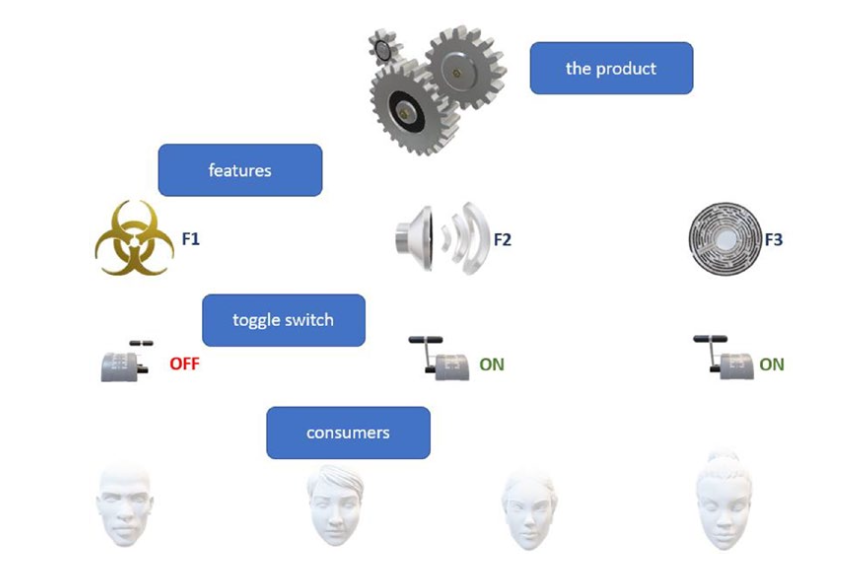
\includegraphics[width=0.6\linewidth]{images/image-04.png}
\end{center}
\end{frame}

% Slide 4: Feature Toggles Use Cases
\begin{frame}
	\frametitle{Feature Toggles Use Cases}
	\begin{itemize}
		\item Activate F1 during Christmas shopping for promotions
		\item Feature changes introduced without code changes
		\item Minimizes risks from system changes
		\item Feature toggles prevent downtime and loss of revenue
		\item Different features can be toggled for different regions
		\item Example: UK gets F1 and F2, US gets F2 and F3
		\item India receives all features (F1, F2, and F3)
	\end{itemize}
\end{frame}

% Slide 5: Engagement with Service Value Chain
\begin{frame}
	\frametitle{Engagement with Service Value Chain}
	\begin{itemize}
		\item Release management involvement across SVC activities
		\item Medium involvement in planning, building, and improving
		\item High involvement in design and transition
		\item Low involvement in engagement and support
		\item Release plans define schedule, types, and techniques
		\item Coordination with Design and Transition activity
		\item Building and testing in Obtain/Build activity
	\end{itemize}
\end{frame}

% Slide 6: Deployment Management Overview
\begin{frame}
	\frametitle{Deployment Management Overview}
	\begin{itemize}
		\item Deployment management in ITIL practices
		\item Deployment: moving software, hardware, or processes to live environments
		\item Not limited to production environments
		\item Includes moving packages to testing and staging environments
		\item Infrastructure deployments included in ITIL 4 scope
		\item Infrastructure as Code (IaC) for cloud infrastructure
		\item Deployments are critical for service delivery
	\end{itemize}
\end{frame}

% Slide 7: Deployment Approaches Overview
\begin{frame}
	\frametitle{Deployment Approaches Overview}
	\begin{itemize}
		\item Multiple deployment approaches based on context
		\item Big bang deployment: all users experience the change simultaneously
		\item Phased deployment: gradual release across regions or features
		\item Continuous delivery/deployment: automated deployment
		\item Pull deployment: users choose when to deploy updates
		\item Each approach has pros and cons
		\item Choice depends on the organization's needs and risks
	\end{itemize}
\end{frame}

% Slide 8: Big Bang and Phased Deployment
\begin{frame}
	\frametitle{Big Bang and Phased Deployment}
	\begin{itemize}
		\item Big bang: all users get updates at the same time
		\item Pilot deployment precedes big bang to ensure readiness
		\item High risk due to simultaneous update
		\item Phased deployment: updates rolled out over time
		\item Allows for learning and correction before full deployment
		\item Geographical or feature-based phased deployment
		\item Phased deployment mitigates risks and manages user impact
	\end{itemize}
\end{frame}

\begin{frame}{deployment approaches}
	 \frametitle{deployment approaches}
\begin{center}
	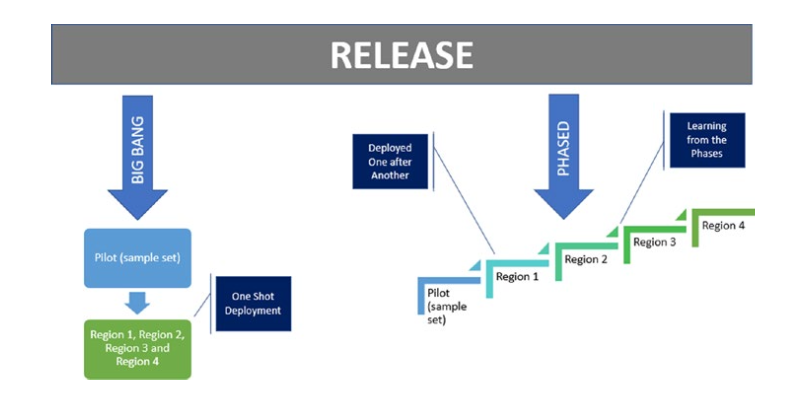
\includegraphics[width=0.6\linewidth]{images/image-05.png}
\end{center}
\end{frame}

% Slide 9: Continuous Delivery/Deployment
\begin{frame}
	\frametitle{Continuous Delivery/Deployment}
	\begin{itemize}
		\item Continuous delivery: manual trigger for production deployment
		\item Continuous deployment: automated deployment to production
		\item Simplicity in no waiting for other parameters
		\item Risk of exposing flaws to end users quickly
		\item Automation plays a key role in deployment pipelines
		\item Requires organizational maturity in DevOps practices
		\item Ensures quick delivery of features to users
	\end{itemize}
\end{frame}

\begin{frame}{Continuous delivery/deployment}
	 \frametitle{Continuous delivery/deployment}
\begin{center}
	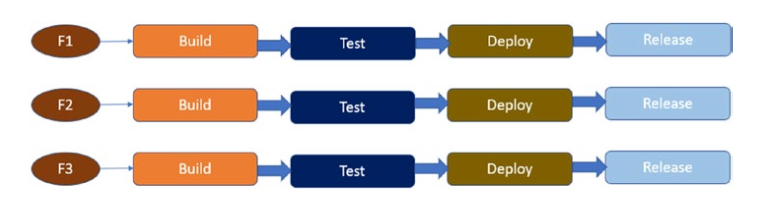
\includegraphics[width=0.8\linewidth]{images/image-06.png}
\end{center}
\end{frame}

% Slide 10: Pull Deployment Overview
\begin{frame}
	\frametitle{Pull Deployment Overview}
	\begin{itemize}
		\item Pull deployment: users choose when to install updates
		\item Software packages available in a repository (DML)
		\item Users notified of available updates
		\item User-triggered installation at their convenience
		\item Effective for minimizing disruption to user productivity
		\item Less common compared to push deployment approaches
		\item Not suitable for urgent security updates
	\end{itemize}
\end{frame}

\begin{frame}{Multiple Choice Question}
\textbf{Which of the following is not a valid type of deployment approach?}

\begin{enumerate}[A.]
	\item Phased deployment
	\item Continuous deployment
	\item Continuous delivery
	\item Emergency deployment
\end{enumerate}
\end{frame}

\end{document}
